\chapter{Popis veličin v prostoru}

\section{Křivkový integrál}

Pokud máme orientovanou po částech hladkou křivku v~prostoru definovanou parametricky pomocí rovnice \eqref{eq:krivkovy_integral_krivka} a~kovariantní vektorové pole \(\kovarvect{v}\), pak křivkový integrál definujeme rovnicí \eqref{eq:krivkovy_integral_definice}.

\begin{equation}
\label{eq:krivkovy_integral_krivka}
\Gamma = (\Gamma^1(t), \Gamma^2(t), ..., \Gamma^n(t)), t \in <t_1, t_2>
\end{equation}

\begin{equation}
\label{eq:krivkovy_integral_definice}
\begin{split}
\int_\Gamma \kovarvect{v} \cdot d\kontravect{l}
\end{split}
\end{equation}

Protože \(\frac{d\kontravect{l}}{dt} = \left(\frac{d \Gamma^1}{dt}, \frac{d \Gamma^2}{dt}, ..., \frac{d \Gamma^n}{dt} \right)\), tak pro parametrickou křivku
\(\Gamma\) platí vztah \eqref{eq:krivkovy_integral_vypocet}.

\begin{equation}
\label{eq:krivkovy_integral_vypocet}
\begin{split}
\int_\Gamma \kovarvect{v} \cdot d\kontravect{l} =
\int_{t_1}^{t_2} \left(\sum_{i=1}^n v_i(\Gamma(t)) \cdot \frac{d \Gamma^i}{dt} \right) dt
\end{split}
\end{equation}

Vidíme, proč vektorové pole \(\kovarvect{v}\) musí být kovariantní. Protože diferenciály souřadnic křivky tvoří kontravariantní vektor, tak pole \(\kovarvect{v}\) musí být kovariantní, aby jejich skalární součin byl invariantní vůči změně soustavy souřadnic. Křivkový integrál je proto také invariantní vůči změně soustavy souřadnic.

Je-li křivka uzavřená (její počáteční a koncový bod jsou shodné), toto zdůrazníme kroužkem přes symbol integrálu, tedy \(\oint_\Gamma \kovarvect{v} \cdot d\kontravect{l}\), a říkáme mu cirkulace vektoru po uzavřené smyčce.

Z definice \eqref{eq:krivkovy_integral_definice} plyne, že integrujeme skalární součin hodnoty pole \(v\) a elementu dráhy \(dl\),
tedy součin průmětu pole do dráhy a elementu dráhy. Křivkový integrál proto lze použít pro výpočet práce, energie a podobně.


\subsection{Příklad}

Elektrické pole má intenzitu \(E = \left(-\frac{y}{x^2+y^2}, \frac{x}{x^2+y^2}\right) \frac{\mathrm{N}}{\mathrm{C}}\). Jakou práci pole vykoná na jednotkovém náboji, který se pohybuje po dráze \(\Gamma(t) = (1, t), t \in <-1, 1>\)?


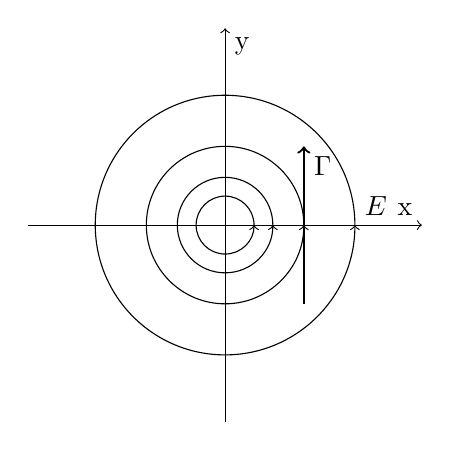
\begin{tikzpicture}
\draw[->] (-2.5, 0) -- (2.5, 0) node[anchor=south east]{x};
\draw[->] (0, -2.5) -- (0, 2.5) node[anchor=north west]{y};

\foreach \r in {0.3679, 0.6065, 1, 1.6487}
	\draw[->, thin] (\r, 0) arc (0:360:\r);
	
\draw (1.65, 0) node[anchor=south west]{\(\vect{E}\)};
	
\draw[->, thick] (1, -1) -- (1, 1) node[anchor=north west]{\(\Gamma\)};
\end{tikzpicture}


Elektrické pole působí na náboj \(Q\) silou \(\vect{F} = \vect{E} \cdot Q\). Práce vykonaná přesunutím náboje \(Q\) po dráze \(\vect{ds}\) je tedy \(dW = \vect{F} \cdot \vect{ds} = \vect{E} \cdot Q \cdot \vect{ds}\) a pro jednotkový náboj \(dW = \vect{E} \cdot \vect{ds}\). Celková práce je tedy

\[
W = \int_{-1}^1 \left (\frac{-t}{1 + t^2} \cdot 0 + \frac{1}{1 + t^2} \cdot 1 \right) = \left[\mathrm{arctg} \ t\right]_{-1}^1 = \frac{\pi}{2} \mathrm{J}
\]

\subsection{Vlastnosti křivkového integrálu}

Nyní vyšetřeme vlastnosti křivkového integrálu. Rovnice \eqref{eq:krivkovy_integral_linearita} udává linearitu křivkového integrálu. Rovnice \eqref{eq:krivkovy_integral_opacny} říká, že křivkový integrál po opačně orientované křivce je opačný. Rovnice \eqref{eq:krivkovy_integral_soucet} udává, že křivkový integrál po křivce, která je rovna součtu dvou křivek, je rovna součtu jejich křivkových integrálů. Oba dva vztahy jsou intuitivní a~lze je snadno ověřit rozepsáním integrálů pomocí vztahu \eqref{eq:krivkovy_integral_vypocet}.

\begin{equation}
\label{eq:krivkovy_integral_linearita}
\begin{split}
\int_{\Gamma} \left(\alpha \kovarvect{u} + \beta \kovarvect{v}\right) \cdot d\kontravect{l} = \alpha \int_{\Gamma} \kovarvect{u} \cdot d\kontravect{l} + \beta \int_{\Gamma} \kovarvect{v} \cdot d\kontravect{l}
\end{split}
\end{equation}

\begin{equation}
\label{eq:krivkovy_integral_opacny}
\begin{split}
\int_{-\Gamma} \kovarvect{v} \cdot d\kontravect{l} = -\int_{\Gamma} \kovarvect{v} \cdot d\kontravect{l}
\end{split}
\end{equation}

\begin{equation}
\label{eq:krivkovy_integral_soucet}
\begin{split}
\int_{\Gamma_1 + \Gamma_2} \kovarvect{v} \cdot d\kontravect{l} = \int_{\Gamma_1} \kovarvect{v} \cdot d\kontravect{l} + \int_{\Gamma_2} \kovarvect{v} \cdot d\kontravect{l}
\end{split}
\end{equation}

Protože skalární součin nezávisí na volbě soustavy souřadnic, tak ani křivkový integrál definovaný vztahem \eqref{eq:krivkovy_integral_definice} nezávisí na volbě soustavy souřadnic. Pro stejné pole a pro stejnou křivku bude křivkový integrál stejný. Je to patrné i z fyzikálního významu. Pokud bude křivkový integrál představovat celkovou práci, pak ta nezávisí na volbě soustavy souřadnic.

Máme-li uzavřenou smyčku \(\Gamma_S\), pak ji můžeme rozdělit na dvě smyčky \(\Gamma_1\) a~\(\Gamma_2\) pomocí libovolně volené přepážky \(\Gamma_P\).

\begin{tikzpicture}
\tikzmath{ \x = 0; \y = 5; }

\draw[->] (\x + 2, \y) arc (0:360:2 and 1);
\draw (\x + 2, \y) node[anchor=west]{\(\Gamma_S\)};

\tikzmath{ \x = 0; \y = 2.5; \t = 0.1; }

\draw[->] (\x + \t, \y - 1) arc (-90:90:2 and 1);
\draw[->] (\x + \t, \y + 1) -- (\x + \t, \y - 0.9);

\draw[->] (\x - \t, \y + 1) arc (90:270:2 and 1);
\draw[->] (\x - \t, \y - 0.9) -- (\x - \t, \y + 1);
\draw (\x, \y) node[anchor=west]{\(\Gamma_P\)};

\draw (\x + \t, \y - 0.9) -- (\x - \t, \y - 0.9);
\draw (\x - \t, \y - 1) -- (\x + \t, \y - 1);

\tikzmath{ \x = 0; \y = 0; \t = 0.1; }

\draw[->] (\x + \t, \y - 1) arc (-90:90:2 and 1);
\draw[->] (\x + \t, \y + 1) -- (\x + \t, \y - 1);
\draw (\x - 2, \y + 0) node[anchor=east]{\(\Gamma_1\)};

\draw[->] (\x - \t, \y + 1) arc (90:270:2 and 1);
\draw[->] (\x - \t, \y - 1) -- (\x - \t, \y + 1);
\draw (\x + 2, \y) node[anchor=west]{\(\Gamma_2\)};
\end{tikzpicture}

Přepážka je tvořena dvěma opačně orientovanými částmi křivky, které jsou nekonečně blízké. Proto se jejich příspěvky do cirkulace vyruší a platí proto vztah \eqref{eq:deleni_cirkulace}. Takto lze cirkulaci vektoru podél křivky rozdělit na součet libovolného počtu cirkulací.

\begin{equation}
\label{eq:deleni_cirkulace}
\begin{split}
\oint_{\Gamma_S} \kovarvect{v} \cdot d\kontravect{l} = \oint_{\Gamma_1} \kovarvect{v} \cdot d\kontravect{l} + \oint_{\Gamma_2} \kovarvect{v} \cdot d\kontravect{l}
\end{split}
\end{equation}

\subsection{Rotace}
\label{sec:rotace}

Vyšetřeme nyní cirkulaci vektoru nekonečně malou smyčkou. Vektorové pole \(\vect{v}\) linearizujeme podle vztahu \eqref{eq:rotace_linearizace}.
Předpokládáme, že pole pole je hladké - má derivace prvního řádu.

\begin{equation}
\label{eq:rotace_linearizace}
\vect{v} \approx \begin{pmatrix}
v_{x_0} + \frac{\partial v_x}{\partial x} \cdot x + \frac{\partial v_x}{\partial y} \cdot y + \frac{\partial v_x}{\partial z} \cdot z \\
v_{y_0} + \frac{\partial v_y}{\partial x} \cdot x + \frac{\partial v_y}{\partial y} \cdot y + \frac{\partial v_y}{\partial z} \cdot z \\
v_{z_0} + \frac{\partial v_z}{\partial x} \cdot x + \frac{\partial v_z}{\partial y} \cdot y + \frac{\partial v_z}{\partial z} \cdot z
\end{pmatrix}
\end{equation}

Dosadíme-li linearizaci \eqref{eq:rotace_linearizace} do vztahu \eqref{eq:krivkovy_integral_vypocet}, získáme vztah \eqref{eq:rotace_1}.

\begin{equation}
\label{eq:rotace_1}
\int_\Gamma \vect{v} \cdot d\vect{l} \approx
\int_{t_1}^{t_2} \begin{pmatrix}
\left(v_{x_0} + \frac{\partial v_x}{\partial x} \cdot \Gamma_x(t) + \frac{\partial v_x}{\partial y} \cdot \Gamma_y(t) + \frac{\partial v_x}{\partial z} \cdot \Gamma_z(t)\right) \cdot \frac{d \Gamma_x}{dt} + \\
\left(v_{y_0} + \frac{\partial v_y}{\partial x} \cdot \Gamma_x(t) + \frac{\partial v_y}{\partial y} \cdot \Gamma_y(t) + \frac{\partial v_y}{\partial z} \cdot \Gamma_z(t)\right) \cdot \frac{d \Gamma_y}{dt} + \\
\left(v_{z_0} + \frac{\partial v_z}{\partial x} \cdot \Gamma_x(t) + \frac{\partial v_z}{\partial y} \cdot \Gamma_y(t) + \frac{\partial v_z}{\partial z} \cdot \Gamma_z(t)\right) \cdot \frac{d \Gamma_z}{dt}
\end{pmatrix} dt
\end{equation}

Úpravou získáme vztah \eqref{eq:rotace_2}.

\begin{equation}
\label{eq:rotace_2}
\begin{matrix}
v_{x_0} \int_{t_1}^{t_2} \frac{d \Gamma_x}{dt} dt + \frac{\partial v_x}{\partial x} \int_{t_1}^{t_2} \Gamma_x(t) \frac{d \Gamma_x}{dt} dt + \frac{\partial v_x}{\partial y} \int_{t_1}^{t_2} \Gamma_y(t) \frac{d \Gamma_x}{dt} dt + \frac{\partial v_x}{\partial z} \int_{t_1}^{t_2} \Gamma_z(t) \frac{d \Gamma_x}{dt} dt + \\
v_{y_0} \int_{t_1}^{t_2} \frac{d \Gamma_y}{dt} dt + \frac{\partial v_y}{\partial x} \int_{t_1}^{t_2} \Gamma_x(t) \frac{d \Gamma_y}{dt} dt + \frac{\partial v_y}{\partial y} \int_{t_1}^{t_2} \Gamma_y(t) \frac{d \Gamma_y}{dt} dt + \frac{\partial v_y}{\partial z} \int_{t_1}^{t_2} \Gamma_z(t) \frac{d \Gamma_y}{dt} dt + \\
v_{z_0} \int_{t_1}^{t_2} \frac{d \Gamma_z}{dt} dt + \frac{\partial v_z}{\partial x} \int_{t_1}^{t_2} \Gamma_x(t) \frac{d \Gamma_z}{dt} dt + \frac{\partial v_z}{\partial y} \int_{t_1}^{t_2} \Gamma_y(t) \frac{d \Gamma_z}{dt} dt + \frac{\partial v_z}{\partial z} \int_{t_1}^{t_2} \Gamma_z(t) \frac{d \Gamma_z}{dt} dt
\end{matrix}
\end{equation}

Vyšetřeme nyní první řádek součtu. Ostatní řádky jsou obdobné.

Integrály \(\int_{t_1}^{t_2} \frac{d \Gamma_x}{dt} dt\) a \(\int_{t_1}^{t_2} \Gamma_x(t) \frac{d \Gamma_x}{dt} dt\) jsou integrály typu \(\int_{t_1}^{t_2} \mathrm{f}(\Gamma_x(t)) \frac{d \Gamma_x}{dt} dt\). Zavedeme-li substituci \(x = \Gamma_x\), tak se integrál redukuje na \(\int_{\Gamma_x(t_1)}^{\Gamma_x(t_2)} \mathrm{f}(x) dx\) a protože je smyčka \(\Gamma\) uzavřená, tak jsou obě integrační meze shodné, tedy \(\Gamma_x(t_1) = \Gamma_x(t_2)\). Proto pro uzavřenou smyčku \(\Gamma\) platí \(\int_{t_1}^{t_2} \mathrm{f}(\Gamma_x(t)) \frac{d \Gamma_x}{dt} dt = 0\).

Dále je tu integrál \(\int_{t_1}^{t_2} \Gamma_z(t) \frac{d \Gamma_x}{dt} dt\). Na obrázku \ref{img:rot_szx} je vidět význam součinu \(\Gamma_y d \Gamma_x\). Jedná se o plochu pod průmětem křivky \(\Gamma\) do roviny \(xz\). Plocha je kladná na pravé části křivky a záporná na levé části. Uvedený integrál tedy představuje kladnou plochu průmětu křivky \(\Gamma\) do roviny \(xz\). Tuto plochu označíme \(S_{xz}\).

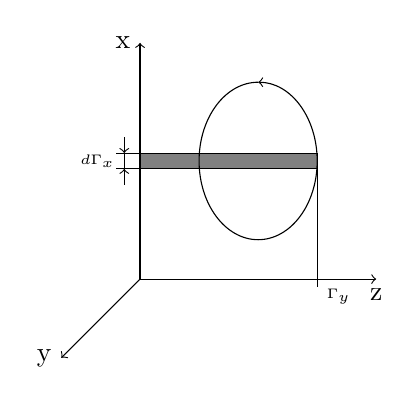
\begin{tikzpicture}
\label{img:rot_szx}
\draw[->] (0, 0) -- (3, 0);
\draw (3, 0) node[anchor=north]{z};

\draw[->] (0, 0) -- (0, 3);
\draw (0, 3) node[anchor=east]{x};

\draw[->] (0, 0) -- (-1, -1);
\draw (-1, -1) node[anchor=east]{y};

\filldraw[color=black, fill=gray] (0, 1.4) -- (2.25, 1.4) -- (2.25, 1.6) -- (0, 1.6) -- (0, 1.4);
\draw[->] (1.5, 2.5) arc (90:450:0.75 and 1);

\draw (0, 1.4) -- (-0.3, 1.4);
\draw (0, 1.6) -- (-0.3, 1.6);

\draw[->] (-0.2, 1.2) -- (-0.2, 1.4);
\draw (-0.2, 1.4) -- (-0.2, 1.6);
\draw (-0.2, 1.5) node[anchor=east]{\tiny \(d \Gamma_x\)};
\draw[->] (-0.2, 1.8) -- (-0.2, 1.6);

\draw (2.25, 1.4) -- (2.25, -0.1);
\draw (2.25, 0) node[anchor=north west]{\tiny \(\Gamma_y\)};
\end{tikzpicture}

Obdobně integrál \(\int_{t_1}^{t_2} \Gamma_y(t) \frac{d \Gamma_x}{dt} dt\) představuje plochu průmětu křivky \(\Gamma\) do roviny \(xy\), tentokrát však zápornou. Označíme ho proto \(-S_{xy}\).

\begin{equation}
\label{eq:rotace_3}
\begin{matrix}
-\frac{\partial v_x}{\partial y} S_{xy} + \frac{\partial v_x}{\partial z} S_{xz} \\
+ \frac{\partial v_y}{\partial x} S_{xy} - \frac{\partial v_y}{\partial z} S_{yz} \\
- \frac{\partial v_z}{\partial x} S_{xz} + \frac{\partial v_z}{\partial y} S_{yz}
\end{matrix}
\end{equation}

Úpravou pak získáme vztah \eqref{eq:rotace_4}.

\begin{equation}
\label{eq:rotace_4}
\left( \frac{\partial v_z}{\partial y} - \frac{\partial v_y}{\partial z} \right) S_{yz} + \left( \frac{\partial v_x}{\partial z} - \frac{\partial v_z}{\partial x} \right) S_{xz} + \left( \frac{\partial v_y}{\partial x} - \frac{\partial v_x}{\partial y} \right) S_{xy} 
\end{equation}

Dále budeme předpokládat, že smyčka leží v rovině (to jsme doposud nemuseli). Označme jednotkovou normálu této roviny \(n\). Pak \(S_{yz} = n_x S\), \(S_{xz} = n_y S\) a \(S_{xy} = n_z S\). Dosazením do vztahu \eqref{eq:rotace_4} získáme vztah \eqref{eq:rotace_5}.

\begin{equation}
\label{eq:rotace_5}
\left( \frac{\partial v_z}{\partial y} - \frac{\partial v_y}{\partial z} \right) n_x S + \left( \frac{\partial v_x}{\partial z} - \frac{\partial v_z}{\partial x} \right) n_y S + \left( \frac{\partial v_y}{\partial x} - \frac{\partial v_x}{\partial y} \right) n_z S 
\end{equation}

Vztah můžeme přepsat na skalární součin \eqref{eq:rotace_6}.

\begin{equation}
\label{eq:rotace_6}
S \cdot \vect{n} \cdot \left(\frac{\partial v_z}{\partial y} - \frac{\partial v_y}{\partial z}, \frac{\partial v_x}{\partial z} - \frac{\partial v_z}{\partial x}, \frac{\partial v_y}{\partial x} - \frac{\partial v_x}{\partial y} \right)
\end{equation}

Vektor na pravé straně skalárního součinu ve vztahu \eqref{eq:rotace_6} závisí pouze na poli \(v\), není závislý na smyčce \(\Gamma\). Nazveme ho rotací pole \(\vect{v}\) a označíme \(\rot \ \vect{v}\). Rotaci tedy lze spočítat posle vztahu \eqref{eq:rotace_vypocet}.

\begin{equation}
\label{eq:rotace_vypocet}
u = \rot \ \vect{v} = \left(\frac{\partial v_z}{\partial y} - \frac{\partial v_y}{\partial z}, \frac{\partial v_x}{\partial z} - \frac{\partial v_z}{\partial x}, \frac{\partial v_y}{\partial x} - \frac{\partial v_x}{\partial y} \right)
\end{equation}

Chceme-li rotaci zapsat ve složkovém tvaru, tak získáme 3 rovnice:

\begin{equation}
\begin{split}
u'_1 = \frac{\partial v'_3}{\partial P'_2} - \frac{\partial v'_2}{\partial P'_3} \\
u'_2 = \frac{\partial v'_1}{\partial P'_3} - \frac{\partial v'_3}{\partial P'_1} \\
u'_3 = \frac{\partial v'_2}{\partial P'_1} - \frac{\partial v'_1}{\partial P'_2}
\end{split}
\end{equation}

Pomocí Levi-Civitova tenzoru \(\varepsilon_{ijk}\) můžeme však všechny 3 rovnice zapsat pomocí jedné.

\begin{equation}
\label{eq:rotace_tenzorova}
\begin{split}
u'_i = \sum_{j=1}^3 \sum_{k=1}^3 \varepsilon_{ijk} \cdot \frac{\partial v'_k}{\partial P'_j}
\end{split}
\end{equation}

Vyjádřeme rotaci v křivočarých souřadnicích. Vztah \eqref{eq:rotace_tenzorova} vypadá, jako dvojí zůžení tenzoru, ale bohužel parciální derivace \(\frac{\partial v_k}{\partial P_j}\) nejsou tenzorem. Vztah tedy misíme upravit tak, aby veličiny v~něm obsažené tenzory byly:

\begin{equation}
\label{eq:rotace_tenzorova_2}
\begin{split}
u'_i = \frac{1}{2} \left(\sum_{j=1}^3 \sum_{k=1}^3 \varepsilon_{ijk} \cdot \frac{\partial v'_k}{\partial P'_j} + \sum_{j=1}^3 \sum_{k=1}^3 \varepsilon_{ijk} \cdot \frac{\partial v'_k}{\partial P'_j} \right) = \\
\frac{1}{2} \left(\sum_{j=1}^3 \sum_{k=1}^3 \varepsilon_{ijk} \cdot \frac{\partial v'_k}{\partial P'_j} + \sum_{k=1}^3 \sum_{j=1}^3 \varepsilon_{ikj} \cdot \frac{\partial v'_j}{\partial P'_k} \right) = \\
\frac{1}{2} \left(\sum_{j=1}^3 \sum_{k=1}^3 \varepsilon_{ijk} \cdot \frac{\partial v'_k}{\partial P'_j} + \sum_{j=1}^3 \sum_{k=1}^3 \varepsilon_{ikj} \cdot \frac{\partial v'_j}{\partial P'_k} \right) = \\
\frac{1}{2} \left(\sum_{j=1}^3 \sum_{k=1}^3 \varepsilon_{ijk} \cdot \frac{\partial v'_k}{\partial P'_j} - \sum_{j=1}^3 \sum_{k=1}^3 \varepsilon_{ijk} \cdot \frac{\partial v'_j}{\partial P'_k} \right) = \\
\frac{1}{2} \sum_{j=1}^3 \sum_{k=1}^3 \varepsilon_{ijk} \cdot \left(\frac{\partial v'_k}{\partial P'_j} - \frac{\partial v'_j}{\partial P'_k} \right)
\end{split}
\end{equation}

V~prvním kroku jsme vztah napsali polovinu dvojnásobku vztahu \eqref{eq:rotace_tenzorova}. Ve druhém kroku jsme provedli substituci \(j \leftrightarrow k\) u~druhého členu - prohodili jsme tyto proměnné. Ve třetím kroku jsme prohodily nezávislé sumy u~druhého členu. Ve čtvrtém kroku jsme prohodily indexy \(j\) a~\(k\), proto jsme museli otočit znaménko u~sumy. Nakonec jsme oba členy spojily. Podle vztahu~\eqref{eq:tenzor_rozdil_derivaci_vektoru} je rozdíl parciálních derivací, který jsme získaly, tenzorem druhého řádu. Rovnice \eqref{eq:rotace_tenzorova_2} je proto tenzorovou rovnicí a~můžeme ji tak proto transformovat:

\begin{equation}
\label{eq:rotace_tenzorova_3}
\begin{split}
u^i = \frac{1}{2} \sum_{j=1}^3 \sum_{k=1}^3 \epsilon^{ijk} \cdot \left(\frac{\partial v_k}{\partial P_j} - \frac{\partial v_j}{\partial P_k} \right) = \\
J' \cdot \frac{1}{2} \sum_{j=1}^3 \sum_{k=1}^3 \varepsilon_{ijk} \cdot \left(\frac{\partial v_k}{\partial P_j} - \frac{\partial v_j}{\partial P_k} \right) = \\
J' \cdot \sum_{j=1}^3 \sum_{k=1}^3 \varepsilon_{ijk} \cdot \frac{\partial v_k}{\partial P_j} = \\
= \sum_{j=1}^3 \sum_{k=1}^3 \epsilon^{ijk} \cdot \frac{\partial v_k}{\partial P_j}
\end{split}
\end{equation}

V~prvním kroku jsme zapsali transformovaný vztah \eqref{eq:rotace_tenzorova_2}, pak jsme rozepsali symbol \(\epsilon_{ijk} = J' \cdot \varepsilon_{ijk}\). Dále jsme využili obdobu vztahu \eqref{eq:rotace_tenzorova_2}, ale obráceně a~pro křivočaré souřadnice. Tento postup nebudu opět opakovat. Nakonec jsme opět přešli k~\(\epsilon\). Vidíme, že rotace transformuje tak, jak bychom čekali. Bez výše uvedeného odvození se však neobejdeme.


\subsection{Stokesova věta}

Mějme plochu \(S\) ohraničenou uzavřenou smyčkou \(\partial S\). Tuto plochu můžeme rozdělit na mnoho malých plošek \(\mathrm{d}S\), které můžeme považovat za rovinné útvary ohraničené uzavřenými křivkami \(\partial \mathrm{d}S\). V sekci \ref{sec:rotace} jsme odvodili vztah \eqref{eq:stokes_ds}.

\begin{equation}
\label{eq:stokes_ds}
\oint_{\partial \mathrm{d}S} \vect{v} \cdot d\vect{l} = (\rot \ \vect{v}) \cdot \vect{n} \cdot ds
\end{equation}

Máme-li 2 sousední plošky, pak se celková cirkulace po jejich vnější hranici sčítá podle vztahu \eqref{eq:deleni_cirkulace}. Jejich příspěvky \((\rot \ \vect{v}) \cdot \vect{n}\) se prostě sčítají. Proto si můžeme dovolit obě strany rovnice \eqref{eq:stokes_ds} integrovat a získáme tak rovnici \eqref{eq:stokesova_veta}. Ta se nazývá Stokesova věta a umožňuje nám přecházet mezi plošným integrálem po ploše \(S\) a křivkovým integrálem po její hranici \(\partial S\).

\begin{equation}
\label{eq:stokesova_veta}
\oint_{\partial S} \vect{v} \cdot d\vect{l} = \int_S (\rot \ \vect{v}) \cdot \vect{n} \cdot ds
\end{equation}


\section{Tok vektoru}

Pokud máme vektorové pole definované v~prostoru, tak můžeme určit jeho tok určenou plochou. Obdobně pokud máme vektorové pole definované
 v~rovině, tak můžeme určit jeho tok určenou křivkou. V~obou případech je tento tok roven integrálu průmětů vektorů pole do normál plochy nebo křivky násobené plochou nebo délkou elementu plochy nebo křivky.
 
Pokud vektorové pole představuje rychlost proudění tekutiny, pak tok vektoru představuje celkový průtok této tekutiny plochou nebo křivkou.

\subsection{Tok vektoru plochou v prostoru - plošný integrál}

Je-li \(S = \left(S_x(t, u), S_y(t, u), S_z(t, u)\right)\) po částech hladká plocha s jednotkovou normálou \(\vect{n}\) a \(\vect{v}\) je vektorové pole,
pak plošný integrál definujeme rovnicí \eqref{eq:plosny_integral_definice}. Říkáme mu tok vektoru \(v\) plochou \(S\).


\begin{equation}
\label{eq:plosny_integral_definice}
\begin{split}
\int_S \vect{v} \cdot d\vect{s} = \int_S \vect{v} \cdot \vect{n} ds
\end{split}
\end{equation}

Využijeme-li vztah \eqref{eq:element_plochy}, tak lze plošný integrál až na znaménko spočítat pomocí vztahu \eqref{eq:plosny_integral_vypocet}.

\begin{equation}
\label{eq:plosny_integral_vypocet}
\begin{split}
\int_S \vect{v} \cdot \vect{n} ds = \iint_S \vect{v} \cdot \left (\frac{\partial S}{\partial t} \times \frac{\partial S}{\partial u}\right) dt \ du
\end{split}
\end{equation}

Je-li plocha uzavřená, pak toto zdůrazníme kroužkem přes symbol integrálu, tedy \(\oint_S \vect{v} \cdot d\vect{s}\). Podle konvence pak normála \(n\) míří vně z plochy.

Například zákon kontinuity toku nestlačitelné kapaliny lze zapsat \(\oint_S \vect{v} \cdot d\vect{s} = 0\). Vyjadřuje fakt, že velkový výtok vektoru rychlosti kapaliny \(v\) jakoukoli uzavřenou plochou \(S\) je nulový, tedy že se kapalina nikde neztrácí, nevyvěrá ani nestlačuje. 

\subsection{Příklad}

Rychlost kapaliny je popsána vztahem \(v = \)

\subsection{Divergence}
\label{sec:divergence}

Vyšetřeme nyní tok vektoru nekonečně malou uzavřenou plochou. Vektorové pole \(\vect{v}\) linearizujeme podle vztahu \eqref{eq:divergence_linearizace}.
Předpokládáme, že pole pole je hladké - má derivace prvního řádu.

\begin{equation}
\label{eq:divergence_linearizace}
\vect{v} \approx \begin{pmatrix}
v_{x_0} + \frac{\partial v_x}{\partial x} \cdot x + \frac{\partial v_x}{\partial y} \cdot y + \frac{\partial v_x}{\partial z} \cdot z \\
v_{y_0} + \frac{\partial v_y}{\partial x} \cdot x + \frac{\partial v_y}{\partial y} \cdot y + \frac{\partial v_y}{\partial z} \cdot z \\
v_{z_0} + \frac{\partial v_z}{\partial x} \cdot x + \frac{\partial v_z}{\partial y} \cdot y + \frac{\partial v_z}{\partial z} \cdot z
\end{pmatrix}
\end{equation}

Dosadíme je do vztahu \eqref{eq:plosny_integral_definice} a získáme tak vztah \eqref{eq:divergence_1}

\begin{equation}
\label{eq:divergence_1}
\begin{split}
\int_S \vect{v} \cdot d\vect{s} = \oint_S \begin{pmatrix}
v_{x_0} + \frac{\partial v_x}{\partial x} \cdot x + \frac{\partial v_x}{\partial y} \cdot y + \frac{\partial v_x}{\partial z} \cdot z \\
v_{y_0} + \frac{\partial v_y}{\partial x} \cdot x + \frac{\partial v_y}{\partial y} \cdot y + \frac{\partial v_y}{\partial z} \cdot z \\
v_{z_0} + \frac{\partial v_z}{\partial x} \cdot x + \frac{\partial v_z}{\partial y} \cdot y + \frac{\partial v_z}{\partial z} \cdot z
\end{pmatrix} \cdot \vect{n} \mathrm{d}s
\end{split}
\end{equation}

Rozepsáním skalárního součinu a integrálu získáme výraz \eqref{eq:divergence_2}.

\begin{equation}
\label{eq:divergence_2}
\begin{matrix}
\int_S \vect{v} \cdot d\vect{s} = \\
v_{x_0} \oint_S n_x \mathrm{d}s + \frac{\partial v_x}{\partial x} \oint_S x n_x \mathrm{d}s + \frac{\partial v_x}{\partial y} \oint_S y n_x \mathrm{d}s + \frac{\partial v_x}{\partial z} \oint_S z n_x \mathrm{d}s + \\
v_{y_0} \oint_S n_y \mathrm{d}s + \frac{\partial v_y}{\partial x} \oint_S x n_y \mathrm{d}s + \frac{\partial v_y}{\partial y} \oint_S y n_y \mathrm{d}s + \frac{\partial v_y}{\partial z} \oint_S z n_y \mathrm{d}s + \\
v_{z_0} \oint_S n_z \mathrm{d}s + \frac{\partial v_z}{\partial x} \oint_S x n_z \mathrm{d}s + \frac{\partial v_z}{\partial y} \oint_S y n_z \mathrm{d}s + \frac{\partial v_z}{\partial z} \oint_S z n_z \mathrm{d}s
\end{matrix}
\end{equation}

Rozeberme první řádek součtu ve výrazu \eqref{eq:divergence_2}. Vyskytují se zde 4 integrály a ve všech se vyskytuje člen \(n_x \mathrm{d}s\). Ten představuje obsah průmětu plochy \(\mathrm{d}s\) do roviny kolmé k ose x, tedy do roviny y-z.

Jednak je zde integrál \(\oint_S x n_x \mathrm{d}s\). Uvědomíme-li si, že \(x n_x \mathrm{d}s\) je objem obecného válce se základnou tvořenou průmětem plochy \(\mathrm{d}s\) do roviny y-z a~výškou \(x\), pak \(\oint_S x n_x \mathrm{d}s = V\) je objem tělesa ohraničeného plochou \(S\).

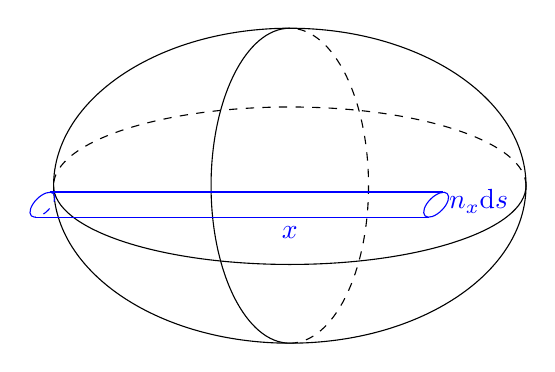
\begin{tikzpicture}
\label{img:objem}

\drawaxes{0}{0}{6}{4}{2}

\draw[thin] (5, 1) arc (0:360:3 and 2);

\draw[dashed] (5, 1) arc (0:180:3 and 1);
\draw[thin] (-1, 1) arc (180:360:3 and 1);

\draw[thin] (2, 3) arc (90:270:1 and 2);
\draw[dashed] (2, -1) arc (270:450:1 and 2);

\draw[color=blue, thin, rotate around={-45:(-1, 0.9)}] (-1, 0.9) arc (90:270:0.1 and 0.2);
\draw[color=blue, dashed, rotate around={-45:(-1, 0.9)}] (-1, 0.9) arc (90:-90:0.1 and 0.2);

\draw[color=blue, thin, rotate around={-45:(4, 0.9)}] (4, 0.9) arc (90:450:0.1 and 0.2);

\draw[color=blue, thin] (-1.05, 0.92) -- (3.95, 0.92);
\draw[color=blue, thin] (-1.23, 0.6) -- (3.77, 0.6);

\draw[color=blue] (3.9, 0.8) node[anchor=west]{\(n_x \mathrm{d}s\)};
\draw[color=blue] (2.0, 0.6) node[anchor=north]{\(x\)};

\end{tikzpicture}

Další 3 integrály jsou typu \(\oint_S f(y, z) n_x \mathrm{d}s\). Uvažujme průmět plochy \(S\) do roviny y-z. Protože je plocha \(S\) uzavřená, tak každým bodem \([y, z]\) projde sudý počet krát, přičemž v polovině případů bude normála plochy orientována v kladném směru osy x, kdy součin \(n_x \mathrm{d}s\) bude kladný, a v polovině případů bude normála plochy orientována v záporném směru osy x, kdy součin \(n_x \mathrm{d}s\) bude záporný. Protože funkce \(f(y, z)\) závisí pouze na souřadnicích \(y\) a \(z\), proto je její funkční hodnota v obou případech stejná a v integrálu se vyruší. Proto \(\oint_S f(y, z) n_x \mathrm{d}s = 0\). Zopakujeme-li uvedený postup pro všechny řádky, získáme vztah \eqref{eq:divergence_3}.

\begin{equation}
\label{eq:divergence_3}
\int_S \vect{v} \cdot d\vect{s} = \frac{\partial v_x}{\partial x} V + \frac{\partial v_y}{\partial y} V + \frac{\partial v_z}{\partial z} V = \left(\frac{\partial v_x}{\partial x} + \frac{\partial v_y}{\partial y} + \frac{\partial v_z}{\partial z}\right) V
\end{equation}
\
Ve výrazu \eqref{eq:divergence_3} se vyskytuje součet, který je závislý pouze na poli \(v\) a nazveme jej divergence pole \(v\). 

\begin{equation}
\label{eq:divergence_definice}
\diverg \vect{v} = \frac{\partial v_x}{\partial x} + \frac{\partial v_y}{\partial y} + \frac{\partial v_z}{\partial z}
\end{equation}

Divergence je definována vztahem \eqref{eq:divergence_definice} a představuje tedy výtok pole \(v\) z nekonečně malého tělesa dělená jeho objemem.

Vyjádřeme divergenci v~křivočarých souřadnicích. Začněme zápisem divergence ve složkovém tvaru:

\begin{equation}
\diverg \vect{v} = \sum_{i=1}^n \frac{\partial v_i}{\partial P'_i}
\end{equation}

Dosadíme-li za derivace vztah \eqref{eq:derivace_vektoru}, získáme:

\begin{equation}
\begin{split}
\diverg \vect{v} = \sum_{i=1}^n \sum_{k=1}^n \sum_{l=1}^n \frac{\partial p_k}{\partial P'_i} \frac{\partial p_l}{\partial P'_i} \frac{\partial v_k}{\partial P_l} + \sum_{i=1}^n \sum_{k=1}^n \frac{\partial^2 p_k}{\partial P'^2_i} v_k = \\
\sum_{k=1}^n \sum_{l=1}^n g^{kl} \frac{\partial v_k}{\partial P_l} + \sum_{i=1}^n \sum_{k=1}^n \frac{\partial^2 p_k}{\partial P'^2_i} v_k = \\
\sum_{k=1}^n \sum_{l=1}^n g^{kl} \frac{\partial v_k}{\partial P_l} + \sum_{k=1}^n v_k \cdot \sum_{i=1}^n \frac{\partial^2 p_k}{\partial P'^2_i}
\end{split}
\end{equation}

\subsection{Vlastnosti toku pole}

Vyšetřeme nyní, jak se chová tok pole při dělení plochy na menší. Mějme uzavřenou plochu \(S_S\), kterou rozdělíme libovolnou přepážkou \(S_P\) na 2 uzavřené plochy \(S_1\) a \(S_2\). Přepážka je tvořena dvěma opačně orientovanými částmi plochy, které jsou nekonečně blízké. Proto se jejich příspěvky do celkového toku vyruší a platí tak vztah \eqref{eq:deleni_toku}.

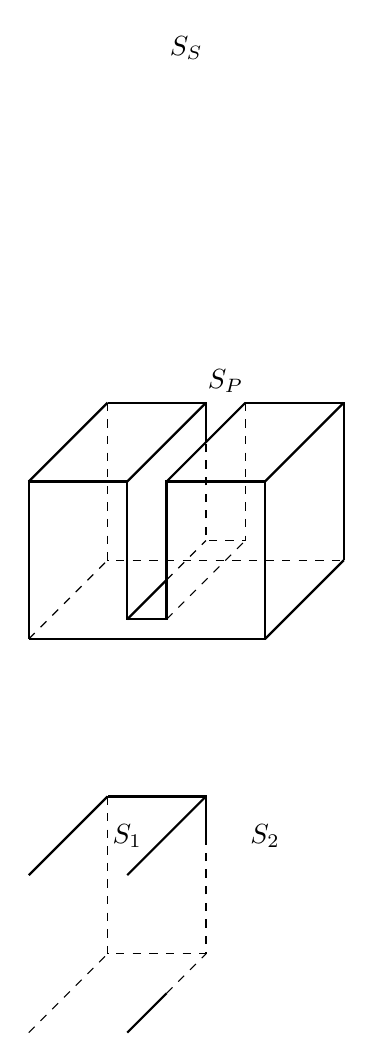
\begin{tikzpicture}
\label{img:deleni_toku}

--== One box ==--

\pgfmathsetmacro{\x}{0}
\pgfmathsetmacro{\y}{10}
\pgfmathsetmacro{\d}{1.0}

\drawaxes{\x}{\y}{4.5}{3}{2}
\drawbox{\x - 0.5}{\y - 1.5}{\x + 2.5}{\y + 0.5}{\d};

\draw (\x + 1.5, \y + 1.0) node[anchor=center]{\(S_S\)};


--== Splitted box ==--

\pgfmathsetmacro{\x}{0}
\pgfmathsetmacro{\y}{5}

\drawaxes{\x}{\y}{4.5}{3}{2}

-- Front
\draw[thick] (\x - 0.5, \y - 1.5) -- (\x + 2.5, \y - 1.5) -- (\x + 2.5, \y + 0.5) -- (\x + 1.25, \y + 0.5) -- (\x + 1.25, \y - 1.25) -- (\x + 0.75, \y - 1.25) -- (\x + 0.75, \y + 0.5) -- (\x - 0.5, \y + 0.5) -- (\x - 0.5, \y - 1.5);

\draw[dashed] (\x - 0.5 + \d, \y + 0.5 + \d) -- (\x - 0.5 + \d, \y - 1.5 + \d) -- (\x + 2.5 + \d, \y - 1.5 + \d);
\draw[thick] (\x + 2.5 + \d, \y - 1.5 + \d) -- (\x + 2.5 + \d, \y + 0.5 + \d) -- (\x + 1.25 + \d, \y + 0.5 + \d);
\draw[dashed] (\x + 1.25 + \d, \y + 0.5 + \d) -- (\x + 1.25 + \d, \y - 1.25 + \d) -- (\x + 0.75 + \d, \y - 1.25 + \d) -- (\x + 0.75 + \d, \y + 0.0 + \d);
\draw[thick] (\x + 0.75 + \d, \y + 0.0 + \d) -- (\x + 0.75 + \d, \y + 0.5 + \d) -- (\x - 0.5 + \d, \y + 0.5 + \d);

\draw[dashed] (\x - 0.5, \y - 1.5) -- (\x - 0.5 + \d, \y - 1.5 + \d);
\draw[thick] (\x + 2.5, \y - 1.5) -- (\x + 2.5 + \d, \y - 1.5 + \d);
\draw[thick] (\x + 2.5, \y + 0.5) -- (\x + 2.5 + \d, \y + 0.5 + \d);
\draw[thick] (\x + 1.25, \y + 0.5) -- (\x + 1.25 + \d, \y + 0.5 + \d);
\draw[dashed] (\x + 1.25, \y - 1.25) -- (\x + 1.25 + \d, \y - 1.25 + \d);
\draw[thick] (\x + 0.75, \y - 1.25) -- (\x + 0.75 + \d / 2, \y - 1.25 + \d / 2);
\draw[dashed] (\x + 0.75 + \d / 2, \y - 1.25 + \d / 2) -- (\x + 0.75 + \d, \y - 1.25 + \d);
\draw[thick] (\x + 0.75, \y + 0.5) -- (\x + 0.75 + \d, \y + 0.5 + \d);
\draw[thick] (\x - 0.5, \y + 0.5) -- (\x - 0.5 + \d, \y + 0.5 + \d);

\draw (\x + 2.0, \y + 1.5) node[anchor=south]{\(S_P\)};


--== Two boxes ==--

\pgfmathsetmacro{\x}{0}
\pgfmathsetmacro{\y}{0}

\drawaxes{\x}{\y}{4.5}{3}{2}

-- Front rectangle
\pgfmathsetmacro{\ax}{\x - 0.5}
\pgfmathsetmacro{\ay}{\y - 1.5}
\pgfmathsetmacro{\bx}{\x + 0.75}
\pgfmathsetmacro{\by}{\y + 0.5}
\drawrect{\ax}{\ay}{\bx}{\by}{thick};

-- Rear rectangle
\draw[dashed] (\ax + \d, \by + \d) -- (\ax + \d, \ay + \d) -- (\bx + \d, \ay + \d) -- (\bx + \d, \y + 1.0);
\draw[thick] (\bx + \d, \y + 1.0) -- (\bx + \d, \by + \d) -- (\ax + \d, \by + \d);

-- Z edges
\draw[dashed] (\ax, \ay) -- (\ax + \d, \ay + \d);
\draw[thick] (\bx, \ay) -- (\bx + \d / 2, \ay + \d / 2);
\draw[dashed] (\bx + \d / 2, \ay + \d / 2) -- (\bx + \d, \ay + \d);
\draw[thick] (\bx, \by) -- (\bx + \d, \by + \d);
\draw[thick] (\ax, \by) -- (\ax + \d, \by + \d);

\drawbox{\x + 1.25}{\y - 1.5}{\x + 2.5}{\y + 0.5}{1.0};

\draw (\x + 0.75, \y + 1.0) node[anchor=center]{\(S_1\)};
\draw (\x + 2.5, \y + 1.0) node[anchor=center]{\(S_2\)};

\end{tikzpicture}


\begin{equation}
\label{eq:deleni_toku}
\oint_{S_S} \vect{v} \cdot \mathrm{d}\vect{s} = \oint_{S_1} \vect{v} \cdot \mathrm{d}\vect{s} + \oint_{S_2} \vect{v} \cdot \mathrm{d}\vect{s}
\end{equation}


\subsection{Gaussův teorém}

Ze vztahu \eqref{eq:divergence_3} můžeme odvodit vztah \eqref{eq:gauss_dv} pro výpočet toku pole elementární uzavřenou ploškou \(\partial \mathrm{d}V\).

\begin{equation}
\label{eq:gauss_dv}
\int_{\partial \mathrm{d}V} \vect{v} \cdot d\vect{s} = \left(\diverg \ \vect{v} \right) \mathrm{d}V
\end{equation}


Podle vztahu \label{eq:deleni_toku} víme, že se toky sousedními ploškami sčítají, přičemž společné části ploch se vyruší. Proto pokud budeme integrovat
vztah \eqref{eq:gauss_dv} přes těleso \(V\), tak plošný integrál přejde na plochu po povrchu tělesa \(V\). Získáme tak Gaussův teorém \eqref{eq:gauss}.

\begin{equation}
\label{eq:gauss}
\oint_{\partial V} \vect{v} \cdot d\vect{s} = \int_V \left(\diverg \ \vect{v} \right) \mathrm{d}V
\end{equation}




\subsection{Tok vektoru křivkou v~rovině}

Je-li \(l = \left(l_x(t), l_y(t)\right)\) po částech hladká plocha s jednotkovou normálou \(\vect{n}\) a \(\vect{v}\) je vektorové pole,
pak tok vektoru \(v\) křivkou \(l\) definujeme rovnicí \eqref{eq:tok_krivkou_definice}.

\begin{equation}
\label{eq:tok_krivkou_definice}
\begin{split}
\int_l \vect{v} \cdot \vect{n} dl
\end{split}
\end{equation}

Máme-li vektor \(d \vect{l} = \left(\frac{d l_x}{dt}, \frac{d l_y}{dt}\right)\), pak vektor k~němu kolmý získáme tak, že prohodíme souřadnice a~u~jedné z~nich otočíme znaménko. Proto \(\vect{n} dl = \left(\frac{d l_y}{dt}, -\frac{d l_x}{dt}\right) dt\). Tok vektoru \(v\) křivkou \(l\) proto můžeme až na znaménko vypočítat podle vztahu \eqref{eq:tok_krivkou_vypocet}.

\begin{equation}
\label{eq:tok_krivkou_vypocet}
\begin{split}
\int_{t_1}^{t_2} \left (v_x \cdot \frac{d l_y}{dt} -v_y \cdot \frac{d l_x}{dt} \right) dt
\end{split}
\end{equation}

\subsection{Greenův teorém}

Obdobou Gaussova teorému v prostoru je Greenův teorém v rovině. Je možné jej odvodit obdobně jako Gaussův teorém.

My jej odvodíme z Gaussova teorému následující úvahou. Nechť je pole \(v\) konstantní ve směru osy \(z\). Těleso \(V\) zvolíme ve formě obecného válce, tedy libovolné podstavy protažené ve směru osy \(z\). Jeho podstavu označme \(S_P\), její hranici \(\partial S_P\) a v výšku válce \(h\).

Vyjděme z Gaussova teorému v rovnici \eqref{eq:green_1}.

\begin{equation}
\label{eq:green_1}
\oint_{\partial V} \vect{v} \cdot d\vect{s} = \int_V \left(\diverg \ \vect{v} \right) \mathrm{d}V
\end{equation}

Tok pole plochou na levé straně rovnice můžeme rozepsat na součet toku pole podstavami a pláštěm válce.
To pláštěm válce je tok hranicí podstavy násobené výškou válce, protože je pole po celé výšce konstantní. Tok podstavami je nulový, protože je pole konstantní ve směru osy \(z\) a tudíž jeho průmět do normály postavy je nulový.

Stejně tak můžeme nahradit objemový integrál na pravé straně rovnice plošným integrálem násobeným výškou. Získáme tak rovnici \eqref{eq:green_2}.

\begin{equation}
\label{eq:green_2}
h \oint_{\partial S_P} \vect{v} \cdot d\vect{l} = h \int_{S_P} \left(\diverg \ \vect{v} \right) \mathrm{d}S
\end{equation}

Podělíme-li rovnici \eqref{eq:green_2} výškou \(h\) a přejmenujeme plochu, tak získáme rovnici \eqref{eq:greenuv_teorem}. Uvědomme si, že \(\frac{\partial v_z}{\partial z} = 0\).
Proto divergence v prostoru, se kterou jsme dosud pracovali, je shodná s divergencí v rovině.

\begin{equation}
\label{eq:greenuv_teorem}
\oint_{\partial S} \vect{v} \cdot d\vect{l} = h \int_S \left(\diverg \ \vect{v} \right) \mathrm{d}S
\end{equation}

Uvedený postup je obecně použitelný, pokud máme problém definovaný v prostoru, ale v jedné nebo více os je invariantní vůči posunutí. Můžeme tak snížit
počet dimenzi problému.

\section{Změna skalárního pole v~daném směru, gradient}

Mějme skalární funkci \(\varphi(P_1, P_2, ..., P_n)\) definovanou obecně v~křivočarých souřadnicích \(P_i\). Chceme-li vypočítat její změnu v~nekonečně blízkém bodě \((P_1 + \mathrm{d}P_1, P_2 + \mathrm{d}P_2, ..., P_n + \mathrm{d}P_n)\), pak
můžeme použít vztah pro totální diferenciál funkce:

\begin{equation}
\begin{split}
\mathrm{d} \varphi = \varphi(P_1 + \mathrm{d}P_1, P_2 + \mathrm{d}P_2, ..., P_n + \mathrm{d}P_n) - \varphi(P_1, P_2, ..., P_n) = \\
\mathrm{d}P_1 \cdot \frac{\partial \varphi}{\partial P_1} + \mathrm{d}P_1 \cdot \frac{\partial \varphi}{\partial P_2} +
... + \mathrm{d}P_n \cdot \frac{\partial \varphi}{\partial P_n} = \\
\sum_{i=1}^n \mathrm{d}P_i \cdot \frac{\partial \varphi}{\partial P_i}
\end{split}
\end{equation}

Kovariantní vektor \(v_i = \frac{\partial \varphi}{\partial P_i}\) nazveme gradientem a~označíme \(\kovarvect{v} = \grad{\varphi}\). Změnu funkční hodnoty pak vypočítáme:

\begin{equation}
\label{eq:zmena_pole_gradient}
\begin{split}
\mathrm{d}\varphi = (\mathrm{d}P_1, \mathrm{d}P_2, ..., \mathrm{d}P_n) \cdot \grad{\varphi} 
\end{split}
\end{equation}

Dále budeme uvažovat pouze kartézský souřadný systém. V~něm víme, že skalární součin dvou vektorů nabývá svého maxima, pokud
mají oba vektory stejný směr. Gradient v~kartézském souřadném systému proto má směr nejvyššího růstu funkce \(\varphi\).

% TODO kolmá konstantní rovina


\section{Operátory}

Dále se seznámíme s operátory, které působí na pole. Již známe operátory divergence a rotace, oba působí na vektorová pole. Divergence vektorového pole
je skalární pole, které má v~každém bodě hodnotu celkového výtoku z~infinitezimálního objemu okolo daného bodu. Rotace je vektorového pole je vektorové
pole, které v každém bodě definuje cirkulaci z nekonečně malých smyček.

Další operátor je gradient. Gradient skalárního pole \(\varphi\) je vektorové pole \(\vect{v}\), které má v~každém bodě směr nejvyššího přírůstku skalárního pole, a velikost rovnou derivaci pole v tomto směru. Je definován vztahem
\[
\vect{v} = \grad \ \varphi = \left(\frac{\partial \varphi}{x}, \frac{\partial \varphi}{y}, \frac{\partial \varphi}{z}\right)
\].

Laplaceův operátor \(\Delta\) přiřazuje skalárnímu poli \(\varphi\) skalární pole \(k\) podle vztahu \(\Delta \varphi = \diverg \ \grad \ \varphi = \frac{\partial^2 \varphi}{\partial x^2} + \frac{\partial^2 \varphi}{\partial y^2} + \frac{\partial^2 \varphi}{\partial z^2}\). Operátor může působit i na vektorové pole, v tom případě působí na každou složku zvlášť. Tedy \(\Delta \ \vect{v} = \left(\Delta \ v_x, \Delta \ v_y, \Delta \ v_z \right) = \left(\frac{\partial^2 v_x}{\partial x^2} + \frac{\partial^2 v_x}{\partial y^2} + \frac{\partial^2 v_x}{\partial z^2},
\frac{\partial^2 v_y}{\partial x^2} + \frac{\partial^2 v_y}{\partial y^2} + \frac{\partial^2 v_y}{\partial z^2},
\frac{\partial^2 v_z}{\partial x^2} + \frac{\partial^2 v_z}{\partial y^2} + \frac{\partial^2 v_z}{\partial z^2} \right)\).

Vektorový Laplaceův operátor je také možné rozepsat na součet vírového a zřídlového pole jak ukazuje rovnice \eqref{eq:vect_laplace_rozepsany}.

\begin{equation}
\label{eq:vect_laplace_rozepsany}
\Delta \ \vect{v} = \grad \ \diverg \ \vect{v} - \rot \ \rot \vect{v} 
\end{equation}

\subsection{Vztahy mezi operátory}

Gradient, divergence, rotace i aplikace laplaceova operátoru jsou lineární operace. Nechť \(\alpha\) a \(\beta\) jsou konstanty, \(\varphi\) a \(rho\) skalární pole a \(u\) a \(v\) vektorová pole. Pak platí tyto vztahy:
\[
\grad(\alpha \cdot \varphi + \beta \cdot \rho) = \alpha \cdot \grad \ \varphi + \beta \cdot \grad \ \rho
\]
\[
\diverg(\alpha \cdot \vect{u} + \beta \cdot \vect{v}) = \alpha \cdot \diverg \ \vect{u} + \beta \cdot \diverg \ \vect{v}
\]
\[
\rot(\alpha \cdot \vect{u} + \beta \cdot \vect{v}) = \alpha \cdot \rot \ \vect{u} + \beta \cdot \rot \ \vect{v}
\]

Tyto vztahy lze jednoduše ověřit dosazením do jejich definic.

Dále jsou důležité následující vztahy mezi operátory.

\begin{equation}
\label{eq:div_rot}
\diverg \ \rot \ \vect{u} = 0
\end{equation}

\begin{equation}
\label{eq:rot_grad}
\rot \ \grad \ \varphi = \vect{0}
\end{equation}

\section{Pole zřídlová a vírová}

Mějme vektorové pole \(\vect{u}\) v prostoru, které má v uvažované oblasti definované derivace prvního řádu. Toto pole má obecně nenulovou divergenci a rotaci.
Pokusíme se toto pole rozložit na součet dvou polí - pole \(\vect{v}\) s nulovou rotací a pole \(\vect{w}\) s nulovou divergencí.

\begin{equation}
\vect{u} = \vect{v} + \vect{w}
\end{equation}

\begin{equation}
\rot \ \vect{v} = \vect{0}
\end{equation}

\begin{equation}
\diverg \ \vect{w} = 0
\end{equation}

To můžeme udělat tak, že stanovíme \(\vect{v} = \grad \ \varphi\). Podmínka nulové rotace je splněna, protože \(\rot \ \vect{v} = \rot \ \grad \ \varphi = \vect{0}\).
Potenciál \(\varphi\) stanovíme tak, aby \(\diverg \ \vect{u} = \diverg \ \vect{v} = \diverg \ \grad \ \varphi\). To je Poissonova rovnice bez okrajových podmínek, která má řešení popsané vztahem \eqref{eq:potencial_v_nekonecnem_prostoru}.

Pole \(\vect{w}\) je tedy \(\vect{w} = \vect{u} - \vect{v}\). Vyšetřeme jeho divergenci. \(\diverg \ \vect{w} = \diverg \ \vect{u} - \diverg \ \vect{v} = \diverg \ \vect{u} - \diverg \ \vect{u} = 0\).

Vidíme, že pole \(u\) je tedy možné rozložit na součet pole s nulovou rotací a pole s nulovou divergencí. Jak uvidíme v sekci \ref{sec:pole_virova}, tak pole
s nulovou divergencí je možné zapsat jako rotaci vektorového potenciálu. Pole \(\vect{u}\) je proto možné rozložit na součet gradientu skalárního potenciálu
a rotace vektorového potenciálu, jak popisuje rovnice \eqref{eq:rozklad_grad_rot}.

\begin{equation}
\label{eq:rozklad_grad_rot}
\vect{u} = \grad \ \varphi + \rot \vect{\psi}
\end{equation}

Podívejme se na obě složky podrobněji.

\subsection{Pole zřídlová}

Mějme pole \(v\), které má v uvažované oblasti nulovou rotaci. Pak podle Stokesovy věty cirkulace vektoru \(v\) všemi uzavřenými smyčkami v uvažované
oblasti je nulová. Mějme v oblasti 2 body A a B. Dále mějme 2 křivky \(\Gamma_1\) a \(\Gamma_2\) které obě začínají v bodě A a končí v bodě B. Pak musí platit rovnost \eqref{eq:potencial_1}. Plyne to z faktu, že otočíme-li jednu z křivek, pak jejich spojením získáme smyčku, která musí mít nulovou cirkulaci.

\begin{equation}
\label{eq:potencial_1}
\int_{\Gamma_1} \vect{v} \cdot d\vect{l} = \int_{\Gamma_2} \vect{v} \cdot d\vect{l}
\end{equation}

To ale znamená, že křivkový integrál potenciálního pole závisí pouze na počátečním a koncovém bodu, ne na tvaru křivky. Dále platí, že křivkové integrály po navazujících křivkách se sčítají. To nám umožňuje zavést skalární pole - potenciál \(\varphi\) splňující podmínku \eqref{eq:potencial_2}. Takováto pole nazýváme zřídlová, potenciální nebo také bezvírová.

\begin{equation}
\label{eq:potencial_2}
\int_{AB} \vect{v} \cdot d\vect{l} = \varphi(\vect{B}) - \varphi(\vect{A})
\end{equation}

Vyšetřeme, jaký je vztah mezi potenciálem \(\varphi\) a polem \(\vect{v}\). Nechť bod \(\vect{B}\) leží v infinitizimálně malé vzdálenosti \(dx\) od bodu
\(\vect{A}\) ve směru osy \(x\). Křivka \(AB\) bude úsečka mezi body \(\vect{A}\) a \(\vect{B}\), má tedy směr osy \(x\). Vztah \eqref{eq:potencial_2} proto lze přepsat do tvaru \eqref{eq:potencial_3}.

\begin{equation}
\label{eq:potencial_3}
\begin{split}
v_x \cdot dx = \varphi(\vect{A} + (dx, 0, 0)) - \varphi(\vect{A}) \\
v_x = \frac{\varphi(\vect{A} + (dx, 0, 0)) - \varphi(\vect{A})}{dx}
\end{split}
\end{equation}

Pro \(dx \rightarrow 0\) získáme vztah \eqref{eq:potencial_4}.

\begin{equation}
\label{eq:potencial_4}
v_x = \frac{\partial \varphi}{\partial x}
\end{equation}

Stejně budeme postupovat pro osy \(y\) a \(z\). Získáme tak vztah \eqref{eq:potencial_5}.

\begin{equation}
\label{eq:potencial_5}
\vect{v} = \left(\frac{\partial \varphi}{\partial x}, \frac{\partial \varphi}{\partial y}, \frac{\partial \varphi}{\partial z}\right) = \grad \ \varphi
\end{equation}

Vidíme tedy, že pole s nulovou rotací lze zapsat jako gradient skalárního potenciálu. Ověřme, že nulová rotace je podmínkou nutnou a postačující pro existenci
potenciálu. Snažíme se tedy dokázat, že pro dané vektorové pole \(v\) existuje potenciál \(\varphi\) takový, že \(\vect{v} = \grad \ \varphi\) tehdy a jen tehdy
pokud \(\rot \ \vect{v} = \vect{0}\).

Podmínku \(\rot \ \vect{v} = \vect{0}\) můžeme rozepsat na \(\frac{\partial v_x}{\partial y} = \frac{\partial v_y}{\partial x}\), \(\frac{\partial v_x}{\partial z} = \frac{\partial v_z}{\partial x}\) a \(\frac{\partial v_y}{\partial z} = \frac{\partial v_z}{\partial y}\).

Že se jedná o podmínku nutnou ověříme snadno. Z definice gradientu plyne \(v_x = \frac{\partial \varphi}{\partial x}\) a \(v_y = \frac{\partial \varphi}{\partial y}\). První rovnici zderivujeme podle \(y\) a získáme \(\frac{\partial v_x}{\partial y} = \frac{\partial^2 \varphi}{\partial x y}\). Druhou rovnici
zderivujeme podle \(x\) a získáme \(\frac{\partial v_y}{\partial x} = \frac{\partial^2 \varphi}{\partial y x}\). Srovnáme-li pravé strany těchto rovnic, pak
díky nezávislosti pořadí derivování jsou shodné. Proto musí platit \(\frac{\partial v_x}{\partial y} = \frac{\partial v_y}{\partial x}\). Obdobně můžeme
postupovat pro ostatní kombinace x-z a y-z a získáme tak zbylé podmínky.

Ověřit, že se jedná o podmínku postačující je poněkud složitější. Rovnice \eqref{eq:potencial_2} nám dává návod, jak potenciál určit. Zvolíme si pevný bod
v oblasti \(A\), v něm zvolíme potenciál \(\varphi_0\). Od tohoto bodu vedeme libovolnou křivku do bodu \(B\), kde hledáme potenciál. Potenciál v něm
pak spočítáme podle vztahu \eqref{eq:potencial_6}. Potenciál \(\varphi\) je tak až na konstantu \(\varphi_0\) plně určen polem \(v\).

\begin{equation}
\label{eq:potencial_6}
\varphi(\vect{B}) = \varphi_0 + \int_{AB} \vect{v} \cdot d\vect{l}
\end{equation}

Abychom ověřili, že tímto postupem skutečně dostaneme potenciál pole \(v\), tak zvolíme takovou křivku \(AB\), která nám umožní snadno spočítat gradient
potenciálu. Za bod \(A\) zvolíme počátek souřadnicového systému. Křivku \(AB\)) vedeme z počátku po ose \(x\) do vzdálenosti \(B_x\), pak ve směru osy
\(y\) do vzdálenosti \(B_y\) a nakonec ve směru osy \(z\) do vzdálenosti \(B_z\), tedy do bodu \(B\). Potenciál je tak určen vztahem \eqref{eq:potencial_7}.

\begin{equation}
\label{eq:potencial_7}
\varphi(\vect{B}) = \varphi_0 + \int_0^{B_x} v_x(x, 0, 0) dx + \int_0^{B_y} v_y(B_x, y, 0) dy  + \int_0^{B_z} v_z(B_x, B_y, z) dz
\end{equation}

Spočítejme nyní parciální derivace potenciálu \(\varphi\). Začněme derivací podle \(z\), přesněji \(B_z\). Na \(B_z\) závisí pouze poslední integrál
integrující podle \(dz\), \(B_z\) se vyskytuje v horní integrační mezi. Derivováním tohoto integrálu proto získáme vztah \eqref{eq:potencial_vz}.

\begin{equation}
\label{eq:potencial_vz}
\frac{\partial \varphi}{B_z} = v_z(B_x, B_y, B_z)
\end{equation}

Pokračujme derivací podle \(y\). \(B_y\) se vyskytuje v horní mezi druhého integrálu a dále ve třetím integrálu. Získáme tak vztah \label{eq:potencial_vy}.
Při jeho úpravě využijeme předpoklad \(\frac{\partial v_y}{\partial z} = \frac{\partial v_z}{\partial y}\).

\begin{equation}
\label{eq:potencial_vy}
\begin{split}
\frac{\partial \varphi}{B_y} = v_y(B_x, B_y, 0) + \int_0^{B_z} \frac{\partial v_z(B_x, B_y, z)}{B_y} dz = \\
v_y(B_x, B_y, 0) + \int_0^{B_z} \frac{\partial v_y(B_x, B_y, z)}{B_z} dz = \\
v_y(B_x, B_y, 0) + v_y(B_x, B_y, B_z) - v_y(B_x, B_y, 0) dz = \\
v_y(B_x, B_y, B_z)
\end{split}
\end{equation}

Nakonec spočítáme derivací podle \(x\). \(B_x\) se vyskytuje v horní mezi prvního integrálu a dále ve druhém a třetím integrálu. Získáme tak vztah \eqref{eq:potencial_vx}. Při jeho úpravě využijeme předpoklady \(\frac{\partial v_x}{\partial z} = \frac{\partial v_z}{\partial x}\) a
\(\frac{\partial v_x}{\partial y} = \frac{\partial v_y}{\partial x}\).

\begin{equation}
\label{eq:potencial_vx}
\begin{split}
\frac{\partial \varphi}{B_x} = v_x(B_x, 0, 0) + \int_0^{B_y} \frac{\partial v_y(B_x, y, 0)}{B_x} dy + \int_0^{B_z} \frac{\partial v_z(B_x, B_y, z)}{B_x} dz = \\
v_x(B_x, 0, 0) + \int_0^{B_y} \frac{\partial v_x(B_x, y, 0)}{B_y} dy + \int_0^{B_z} \frac{\partial v_x(B_x, B_y, z)}{B_z} dz = \\
v_x(B_x, 0, 0) + v_x(B_x, B_y, 0) - v_x(B_x, 0, 0) + v_x(B_x, B_y, B_z) - v_x(B_x, B_y, 0) = \\
v_x(B_x, B_y, B_z)
\end{split}
\end{equation}

Vidíme, že všechny parciální derivace potenciálu odpovídají složkám gradientu. Dokázali jsme tak, že má-li pole \(v\) nulovou rotaci, můžeme zavést jeho
potenciál vztahem \eqref{eq:potencial_7} a díky vztahu \eqref{eq:potencial_1} obecně vztahem \eqref{eq:potencial_6}.

\subsection{Pole vírová}
\label{sec:pole_virova}

Vektorová pole \(\vect{v}\) mající v celé uvažované oblasti nulovou divergenci nazýváme pole vírová. Takováto pole můžeme zapsat ve formě 
\eqref{eq:virova_pole_definice}. Veličinu \(\vect{\psi}\) nazýváme vektorovým potenciálem pole \(\vect{v}\).

\begin{equation}
\label{eq:virova_pole_definice}
\vect{v} = \rot \ \vect{\psi}
\end{equation}

Ze vztahu \eqref{eq:div_rot} je zřejmé, že nulová divergence pole \(\vect{v}\) je podmínkou nutnou pro existenci vektorového potenciálu. Že se jedná o podmínku postačující a jak potenciál určit uvidíme dále.

Z rovnice \eqref{eq:virova_pole_nejednoznacnost} je vidět, že vektorový potenciál není polem \(\vect{v}\) určen jednoznačně.
Můžeme k němu přičíst libovolné pole s nulovou rotací, tedy libovolné potenciální pole, a rovnice \eqref{eq:virova_pole_definice}
zůstane v platnosti.

\begin{equation}
\label{eq:virova_pole_nejednoznacnost}
\rot \left(\vect{\psi} + \grad \varphi \right) = \rot \ \vect{\psi} + \rot \ \grad \varphi =
\rot \ \vect{\psi} + \vect{0} = \rot \ \vect{\psi}
\end{equation}

Speciálním případem je situace, kdy \(\varphi\) zvolíme tak, že \(\diverg \vect{\psi} + \diverg \grad \varphi = 0\). To bude splněno pokud
\(-\diverg \vect{\psi} = \diverg \grad \varphi = 0\). Pravá strana rovnice představuje Poissonovu rovnici bez okrajových podmínek.
Její řešení je uvedeno dále, ale nyní je podstatná pouze jeho existence. Důsledkem tedy je, že existuje-li pole \(\vect{\psi}\) řešící
rovnici \eqref{eq:virova_pole_definice}, pak existuje \(\vect{\psi}\) takové, že má nulovou divergenci, tedy vírové pole.

Vyjdeme z rovnice \eqref{eq:virova_pole_definice}. Beze ztráty na obecnosti můžeme potenciál \(\varphi\) považovat za vírové pole.
Zaveďme tedy potenciál \(\vect{\rho}\) vztahem \(\vect{\psi} = \rot \ \vect{\rho}\). Abychom určili potenciál \(\vect{\rho}\), tak tedy
potřebujeme vyřešit rovnici \eqref{eq:virova_pole_potencial_1}.

\begin{equation}
\label{eq:virova_pole_potencial_1}
\vect{v} = \rot \ \rot \ \vect{\rho}
\end{equation}

Jak jsme viděli výše, tak můžeme zavést podmínku \(\diverg \ \vect{\rho} = 0\). Pak ale můžeme k rovnici \eqref{eq:virova_pole_potencial_1}
přičíst \(\grad \ \diverg \ \vect{\rho}\), který je nulový. Dále ještě rovnici invertujeme. Získáme tak rovnici \eqref{eq:virova_pole_potencial_2}.

\begin{equation}
\label{eq:virova_pole_potencial_2}
-\vect{v} = \grad \ \diverg \ \vect{\rho} - \rot \ \rot \ \vect{\rho}
\end{equation}

Pravou stranu rovnice můžeme přepsat podle vztahu \eqref{eq:vect_laplace_rozepsany}, získáme tak rovnici \eqref{eq:virova_pole_potencial_3}.

\begin{equation}
\label{eq:virova_pole_potencial_3}
-\vect{v} = \Delta \ \vect{\rho}
\end{equation}

To je vektorová Poissonova rovnice bez okrajových podmínek. Jak uvidíme dále, tak tato rovnice má řešení. Proto vírová pole \(v\) lze vyjádřit
pomocí pomocí rovnice \eqref{eq:virova_pole_definice} a to tak, že vyřešíme rovnici \eqref{eq:virova_pole_potencial_3} a dopočítáme \(\vect{psi} = \rot \ \vect{rho}\).

